\documentclass[11pt, a4paper]{article}
\usepackage[utf8]{inputenc}
\usepackage[T1]{fontenc}
\usepackage[brazilian]{babel}
\usepackage{lmodern}
\usepackage{setspace}
\usepackage{geometry}
\usepackage{indentfirst}
\usepackage{microtype}
\usepackage{enumitem}
\usepackage{graphicx}
\usepackage{array}
\usepackage{longtable}
\usepackage{booktabs}

% Margens calibradas para que a Parte 1 ocupe exatamente a Página 1
\geometry{a4paper, left=2.2cm, right=2cm, top=1.4cm, bottom=1.4cm}
\setlength{\parindent}{1.0cm}
\setlength{\parskip}{0.03cm}
\renewcommand{\arraystretch}{1.26}

\begin{document}
\pagestyle{empty}

% ============================================================================
% PARTE 1: DOCUMENTO TEXTUAL DE UMA PÁGINA (DESCRIÇÃO GERAL DO CONTEXTO)
% ============================================================================
\begin{spacing}{0.85}
\setlength{\parskip}{0.02cm}

\begin{center}
    {\large\bfseries AGENTE INTELIGENTE PARA MONITORAMENTO DA QUALIDADE DO AR EM SMART CAMPUS}\\[0.08cm]
    {\small\textbf{Autor:} Noedson Romario Vieira da Silva \quad|\quad \textbf{PPCA -- NDAE/UFPA}}
    \vspace{0.04cm}
    \hrule
\end{center}

\vspace{0.04cm}

\noindent\textbf{1. Propósito Geral}\par
O sistema desenvolvido é uma plataforma autônoma de ponta a ponta (Borda-Nuvem) 
voltada ao monitoramento contínuo, previsão temporal e diagnóstico inteligente da qualidade do ar
em ambientes internos (como laboratórios e salas de aula) 
e externos de um \emph{Smart Campus} na região amazônica. Diferentemente 
das soluções convencionais de Internet das Coisas (IoT) --- que operam de
maneira puramente passiva, limitando-se a coletar medições e exibi-las em painéis 
estáticos após o ambiente já se encontrar poluído ---, este sistema atua como um 
Agente Inteligente Proativo. Sua função primordial é 
proteger a saúde dos ocupantes do campus antecipando episódios críticos de contaminação 
atmosférica com 15 minutos de antecedência, ao mesmo 
tempo em que audita automaticamente a integridade física dos próprios sensores instalados em campo.

\vspace{0.04cm}
\noindent\textbf{2. Coleta e Transmissão de Dados Ambientais em Tempo Real:}\par
Na prática, o sistema monitora continuamente sete compostos gasosos
por meio de estações sensoras de baixo custo equipadas com os sensores semicondutores 
\emph{MQ-135} e \emph{MQ-131}, aferindo as concentrações de 
monóxido de carbono (CO), dióxido de carbono (CO\textsubscript{2}), amônia (NH\textsubscript{4}), álcool, 
acetona, tolueno e ozônio (O\textsubscript{3}). Cada estação física baseia-se no microcontrolador 
\emph{Heltec WiFi LoRa 32 v2} gerenciado pelo sistema operacional de tempo real \emph{FreeRTOS}, 
garantindo leituras periódicas determinísticas sem perda de pacotes. Para vencer grandes distâncias no 
campus universitário com baixo consumo de energia e sem depender de cobertura Wi-Fi local, as 
estações transmitem os pacotes via rádio LoRaWAN (padrão brasileiro 
\texttt{AU915\_0}) até um \emph{gateway} central --- contando também com um modo de simulação 
integrado (\emph{LWN-Simulator}) que emula estações virtuais para validação completa antes da 
implantação física.

\vspace{0.04cm}
\noindent\textbf{3. Recepção, Adequação à Norma Ambiental e Armazenamento Centralizado:}\par
Ao chegarem ao servidor de rede ChirpStack v4, 
os pacotes LoRaWAN são autenticados, decodificados automaticamente em 
valores numéricos de concentração (ppm) e enviados diretamente à plataforma web central 
desenvolvida em Python/Django. O sistema armazena cada leitura no banco de dados 
relacional PostgreSQL, vinculando-a à identificação única da estação (\texttt{DevEUI}), 
sua localização e o instante exato da coleta. Em seguida, o sistema realiza o processamento 
científico dos sinais: agrega as leituras em médias de 1 minuto (eliminando ruídos 
elétricos de alta frequência típicos de sensores de baixo custo), organiza uma janela histórica 
recente de 30 minutos e calcula a 
média móvel das últimas 8 horas de monóxido de carbono (CO), 
cumprindo estritamente o critério oficial da legislação ambiental brasileira 
(Resolução CONAMA nº 491/2018) e da agência norte-americana US-EPA.

\vspace{0.04cm}
\noindent\textbf{4. Inteligência Artificial Embarcada (As Três Entregas do Agente Inteligente):}\par
A cada nova leitura recebida, o Agente Inteligente integrado ao servidor 
(baseado em uma Rede Neural Recorrente \emph{Bidirectional LSTM Multi-Task} em \emph{TensorFlow/Keras}) 
analisa o comportamento temporal dos gases e executa simultaneamente três ações autônomas:
\begin{enumerate}[nosep, leftmargin=1.4cm, topsep=0.02cm]
    \item \textbf{Previsão Futura de Poluentes (\emph{Forecasting} de 15 minutos):} estima quantitativamente qual será a concentração de cada um dos sete gases \textbf{15 minutos à frente}, permitindo identificar tendências de elevação brusca antes que limites nocivos à saúde sejam atingidos;
    \item \textbf{Classificação Preventiva do Índice de Qualidade do Ar (IQAr):} enquadra a condição futura do ar (em 15 minutos) nas classes normativas \textbf{Boa} ($< 4{,}5\textrm{ ppm}$), \textbf{Moderada} ($4{,}5\textrm{ a }9{,}5\textrm{ ppm}$) ou \textbf{Ruim} ($\ge 9{,}5\textrm{ ppm}$), emitindo avisos preventivos antecipados para tomada de decisão e ventilação ou evacuação do local;
    \item \textbf{Autodiagnóstico de Falhas e Anomalias nos Sensores:} verifica a confiabilidade dos próprios equipamentos combinando um \emph{Autoencoder} neural (que detecta picos elétricos espúrios e perda gradual de calibração) com um monitor estatístico de variância temporal ($\sigma < \epsilon$) que detecta imediatamente se um sensor \textbf{travou ou congelou} enviando valores constantes repetidos, impedindo que falhas eletrônicas gerem falsos alertas ambientais.
\end{enumerate}

\vspace{0.04cm}
\noindent\textbf{5. Emissão Inteligente de Alertas e Suporte à Decisão:}\par
Por fim, todas as medições atuais, projeções futuras de 15 minutos, probabilidades de risco do IQAr e diagnósticos de saúde dos sensores são registrados e exibidos em tempo real em painéis analíticos e APIs web. Quando o Agente detecta uma falha física no sensor ou prevê qualidade do ar ``Ruim'', ele dispara automaticamente um \textbf{alerta estruturado} --- regulado por um intervalo inteligente de segurança (\emph{cooldown} de 15 minutos) para evitar alertas duplicados ---, entregando ao campus um sistema completo, preventivo e autônomo de gestão da qualidade do ar.

\end{spacing}

% ============================================================================
% PARTE 2: DIAGRAMA DE CASOS DE USO (FERRAMENTA CASE ASTAH)
% ============================================================================
\newpage
\pagestyle{plain}
\setcounter{page}{2}
\setlength{\parindent}{0pt}
\setlength{\parskip}{0.2cm}

\begin{center}
    {\Large\bfseries DIAGRAMA DE CASOS DE USO (UML)}\\[0.1cm]
    {\normalsize Modelado na ferramenta CASE \textbf{Astah}}
    \vspace{0.1cm}
    \hrule
\end{center}

\vspace{0.2cm}

A Figura 1 apresenta o Diagrama de Casos de Uso do \textbf{Sistema IQArMobi}, elaborado na ferramenta CASE \textbf{Astah} conforme a notação UML. O modelo contempla \textbf{três atores externos} (\emph{Servidor Chirpstack}, \emph{Gestor Ambiental/Usuário} e \emph{Administrador do Sistema}) e \textbf{sete casos de uso}, articulando relacionamentos de associação, inclusão obrigatória (\texttt{<<include>>}) e extensão condicional (\texttt{<<extend>>}).

\begin{figure}[htbp]
    \centering
    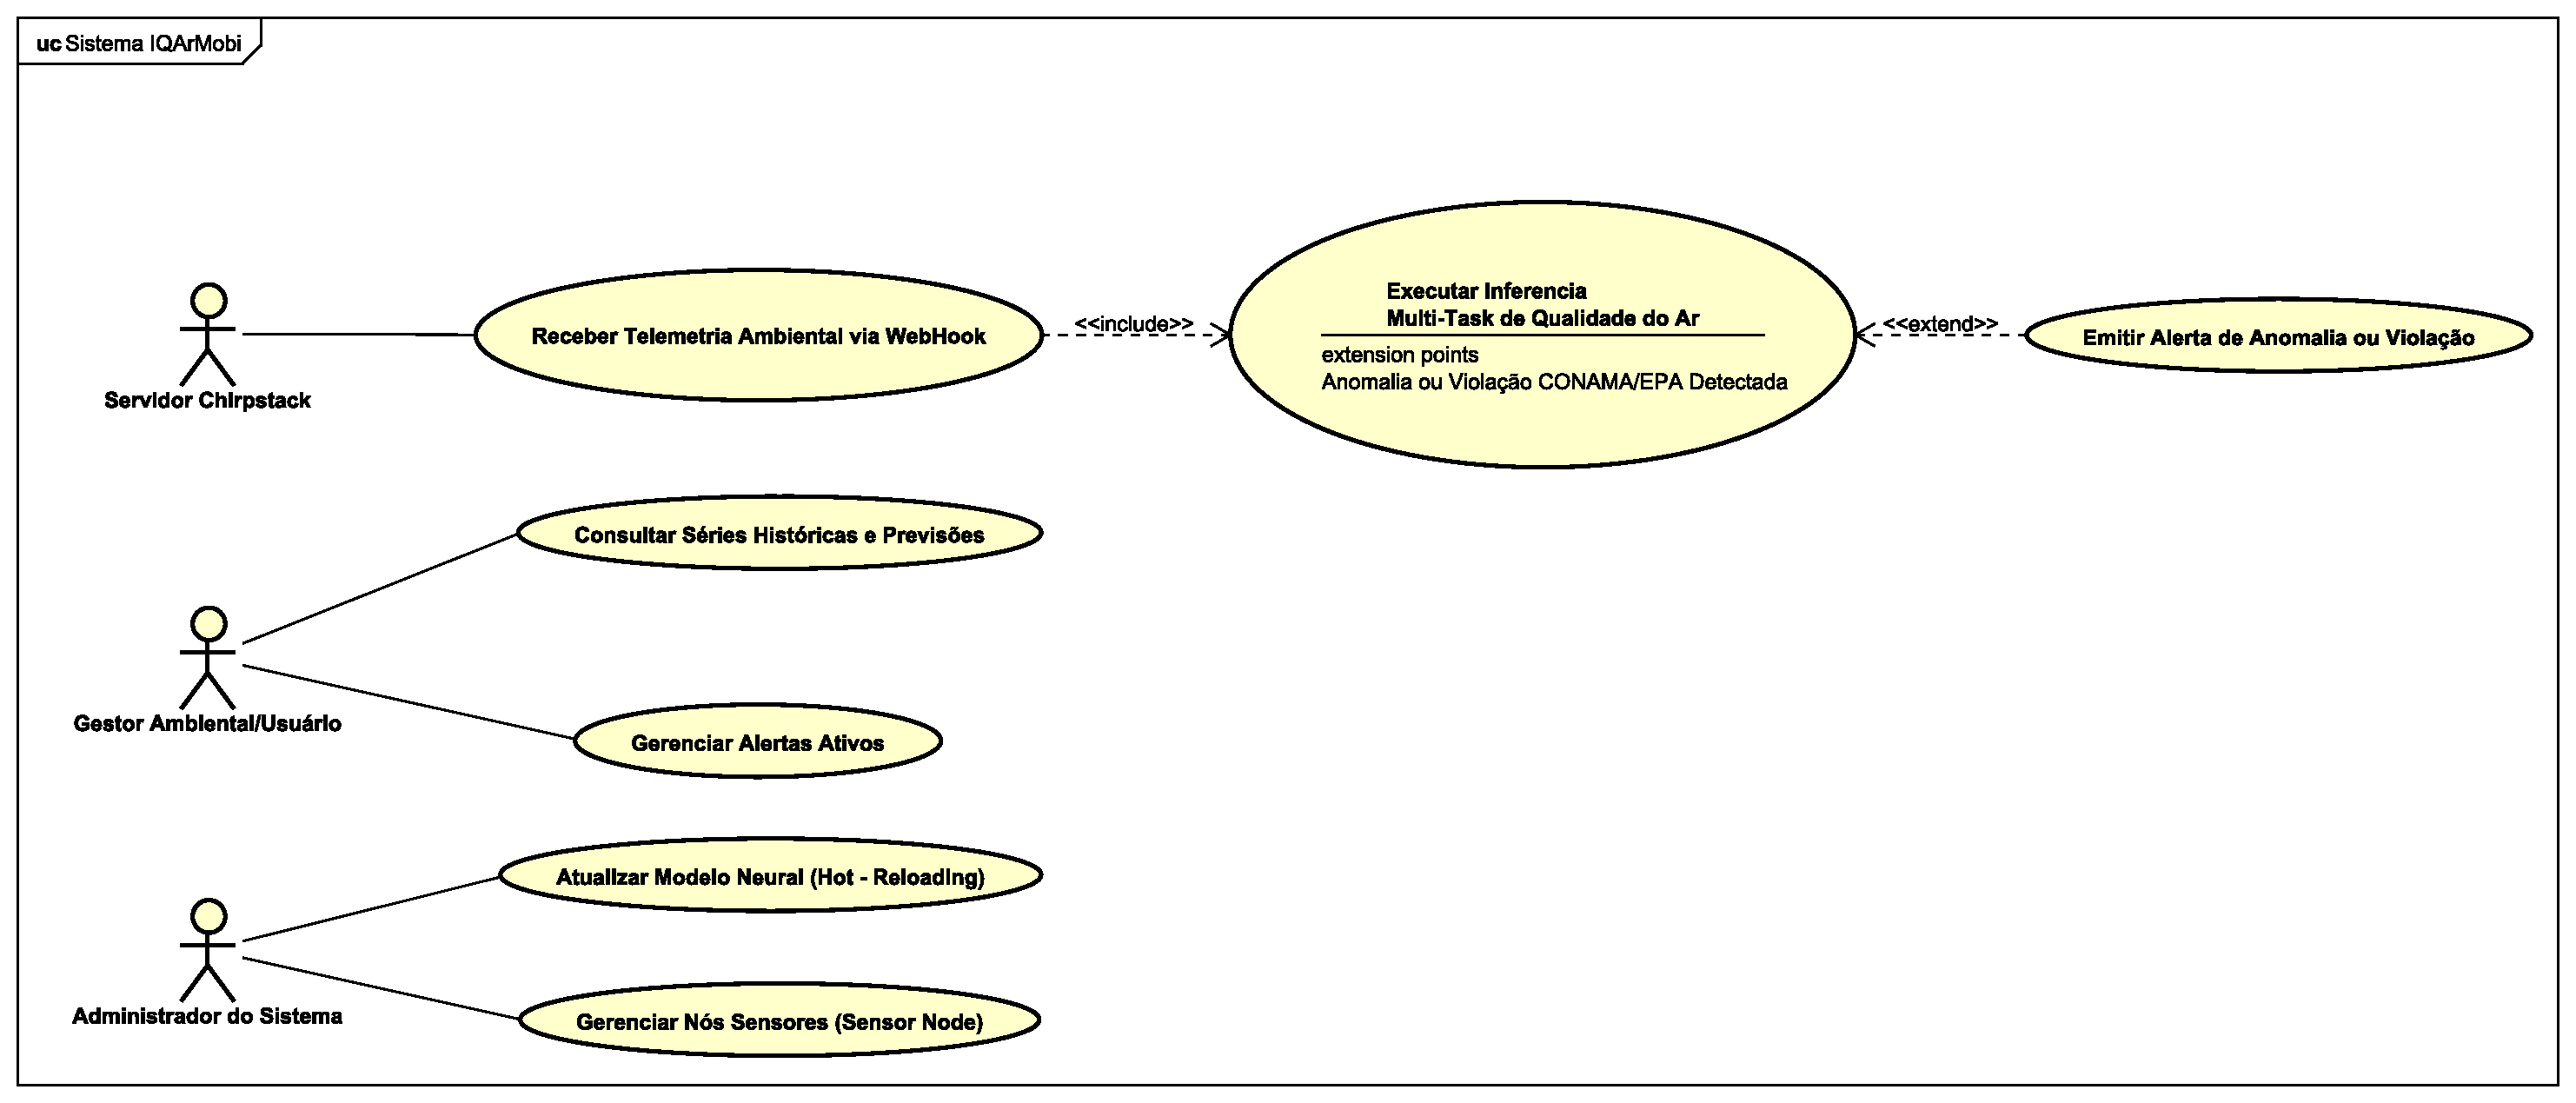
\includegraphics[width=1.0\textwidth]{diagrama_casos_de_uso.pdf}
    \caption{Diagrama de Casos de Uso do Sistema IQArMobi modelado no Astah.}
    \label{fig:uc_diagram}
\end{figure}

\subsection*{Síntese dos Elementos do Diagrama}
\begin{itemize}[nosep, leftmargin=0.6cm]
    \item \textbf{Servidor Chirpstack (Ator Externo --- Sistema):} Servidor de rede LoRaWAN que decodifica os pacotes enviados pelas estações sensoras de campo e aciona o caso de uso \emph{Receber Telemetria Ambiental via WebHook} (\texttt{UC01}).
    \item \textbf{Gestor Ambiental / Usuário (Ator Humano):} Responsável por monitorar o ambiente universitário por meio dos casos de uso \emph{Consultar Séries Históricas e Previsões} (\texttt{UC04}) e \emph{Gerenciar Alertas Ativos} (\texttt{UC05}).
    \item \textbf{Administrador do Sistema (Ator Humano):} Responsável pela manutenção operacional e atualização do Agente Inteligente por meio dos casos de uso \emph{Atualizar Modelo Neural (Hot - Reloading)} (\texttt{UC06}) e \emph{Gerenciar Nós Sensores (Sensor Node)} (\texttt{UC07}).
    \item \textbf{Relacionamentos de Inclusão e Extensão:} A recepção de telemetria (\texttt{UC01}) inclui obrigatoriamente (\texttt{<<include>>}) o caso de uso \emph{Executar Inferência Multi-Task de Qualidade do Ar} (\texttt{UC02}), o qual é estendido opcionalmente (\texttt{<<extend>>}) pelo caso de uso \emph{Emitir Alerta de Anomalia ou Violação} (\texttt{UC03}) quando o ponto de extensão \emph{``Anomalia ou Violação CONAMA/EPA Detectada''} é satisfeito.
\end{itemize}

% ============================================================================
% PARTE 3: MODELO DE CASOS DE USO TEXTUAL
% ============================================================================
\newpage

\begin{center}
    {\Large\bfseries ESPECIFICAÇÃO TEXTUAL DO MODELO DE CASOS DE USO}\\[0.1cm]
    {\normalsize Formato estruturado conforme definido na vídeo-aula da disciplina}
    \vspace{0.1cm}
    \hrule
\end{center}

\vspace{0.15cm}

A seguir são detalhadas as especificações textuais dos casos de uso do \textbf{Sistema IQArMobi}, contemplando os campos definidos na vídeo-aula: \emph{Identificador}, \emph{Nome}, \emph{Breve Descrição}, \emph{Atores e Participação}, \emph{Prioridade}, \emph{Pré-condições}, \emph{Pós-condições}, \emph{Fluxo de Eventos Principal}, \emph{Subfluxos}, \emph{Fluxos Secundários/Exceções} e \emph{Requisitos Não Funcionais Associados}.

% --- UC01 ---
\subsection*{1. Especificação do Caso de Uso}

\begin{longtable}{|>{\bfseries}p{3.8cm}|p{12.2cm}|}
\hline
\multicolumn{2}{|c|}{\textbf{Receber Telemetria Ambiental via WebHook}} \\ \hline


Nome & Receber Telemetria Ambiental via WebHook \\ \hline

Breve Descrição & 
Permite que o sistema receba automaticamente os pacotes de telemetria dos sete compostos 
gasosos enviados pelo servidor de rede LoRaWAN, valide e armazene as leituras ambientais, acione 
obrigatoriamente a inferência de Inteligência Artificial e, caso seja detectada anomalia física ou 
risco ambiental, dispare um alerta preventivo. \\ \hline

Atores & 
\begin{minipage}[t]{\linewidth}
\vspace{0.05cm}
\begin{tabular}{@{}p{4.0cm}p{7.8cm}@{}}
\textbf{Ator} & \textbf{Como participa do Caso de Uso} \\ \hline
\emph{Servidor Chirpstack} (Ator Primário / Sistema Externo) & Inicia o caso de uso enviando uma notificação HTTP (WebHook) contendo a identificação da estação sensora (\texttt{DevEUI}) e as concentrações decodificadas dos gases em ppm. \\
\end{tabular}
\vspace{0.1cm}
\end{minipage} \\ \hline

Casos de Uso Relacionados & 
\begin{itemize}[nosep, leftmargin=0.5cm]
    \item \textbf{\texttt{<<include>>} (Executar Inferência Multi-Task de Qualidade do Ar):} executado obrigatoriamente a cada nova leitura válida recebida.
    \item \textbf{\texttt{<<extend>>} (Emitir Alerta de Anomalia ou Violação):} executado opcionalmente quando o ponto de extensão \emph{``Anomalia ou Violação CONAMA/EPA Detectada''} é atingido após a inferência.
\end{itemize} \\ \hline

Prioridade & \textbf{Essencial (Alta)} \\ \hline

Pré-condições & 
\begin{enumerate}[nosep, leftmargin=0.5cm]
    \item A estação sensora emissora deve estar previamente cadastrada e ativa no sistema.
    \item O modelo neural \emph{Multi-Task} e os normalizadores devem estar carregados em memória pelo Agente Inteligente.
\end{enumerate} \\ \hline

Pós-condições & 
\begin{enumerate}[nosep, leftmargin=0.5cm]
    \item A nova leitura ambiental dos sete gases é registrada no histórico do sistema.
    \item A previsão futura (15 minutos à frente), a classificação do Índice de Qualidade do Ar (IQAr) e o diagnóstico de integridade do sensor são salvos e disponibilizados nos painéis.
    \item Se houver risco ambiental ou falha física do sensor, um registro de alerta ativo é gerado.
\end{enumerate} \\ \hline

Fluxo de Eventos Principal (Caminho Feliz) & 
\begin{enumerate}[nosep, leftmargin=0.5cm]
    \item O Servidor Chirpstack envia ao sistema um evento de telemetria (\texttt{up}) contendo o identificador da estação (\texttt{DevEUI}) e as medições dos sete gases (CO, CO\textsubscript{2}, NH\textsubscript{4}, álcool, acetona, tolueno e O\textsubscript{3}).
    \item O Sistema verifica a autenticidade do evento, identifica a estação sensora correspondente e registra a leitura ambiental no banco de dados.
    \item O Sistema agrega as leituras em janela temporal de 30 minutos (com médias de 1 minuto) e calcula a média móvel de 8 horas de monóxido de carbono (CO).
    \item O Sistema inclui e executa o caso de uso Executar Inferência Multi-Task de Qualidade do Ar, obtendo: (a) as concentrações previstas para os próximos 15 minutos, (b) a classificação normativa do IQAr (\emph{Boa}, \emph{Moderada} ou \emph{Ruim}) e (c) o diagnóstico de saúde física do sensor.
    \item O Sistema armazena os resultados da inferência vinculados à estação sensora.
    \item O Sistema retorna a confirmação de recebimento e processamento com sucesso (\texttt{HTTP 200 OK}) ao Servidor Chirpstack, encerrando o caso de uso.
\end{enumerate} \\ \hline

Fluxos Secundários (Alternativos e de Exceção) & 
\begin{itemize}[nosep, leftmargin=0.5cm]
    \item \textbf{[Fluxo Alternativo / Extensão no Passo 4 --- Violação Ambiental ou Anomalia no Sensor]:} Caso o resultado da inferência indique qualidade do ar futura \emph{``Ruim''} ($\ge 9{,}5\textrm{ ppm}$) ou falha física no sensor (erro de reconstrução elevado ou sinal congelado com variância nula), o sistema aciona a extensão  Emitir Alerta de Anomalia ou Violação, verifica se não há alerta idêntico emitido nos últimos 15 minutos (\emph{cooldown}) e registra um novo alerta crítico antes de prosseguir para o Passo 5.
    \item \textbf{[Exceção no Passo 2 --- Evento de Controle sem Carga de Telemetria]:} Caso o Servidor Chirpstack envie um pacote apenas de controle de rede (como confirmação de conexão \emph{join} ou status de bateria) sem leituras de gases, o sistema ignora a etapa de inferência, registra apenas o status de comunicação e retorna confirmação ao servidor.
    \item \textbf{[Exceção no Passo 3 --- Histórico Insuficiente na Inicialização (\emph{Cold Start})]:} Caso a estação sensora tenha acabado de ser ligada e ainda possua menos de 30 minutos de histórico acumulado, o sistema armazena a leitura atual, preenche temporariamente a janela histórica e sinaliza que a previsão opera em regime inicial.
\end{itemize} \\ \hline

Requisitos Não Funcionais Associados & 
\begin{itemize}[nosep, leftmargin=0.5cm]
    \item \textbf{Desempenho (Tempo de Resposta):} O processamento completo (recepção, inferência neural das três tarefas e gravação) deve ocorrer em tempo inferior a 500 milissegundos por requisição.
    \item \textbf{Concorrência e Disponibilidade:} O carregamento do modelo neural em memória deve ser único e protegido contra condições de corrida (\emph{Thread-Safe}), suportando múltiplas estações transmitindo simultaneamente.
\end{itemize} \\ \hline
\end{longtable}

% --- UC04 ---
\subsection*{2. Especificação do Caso de Uso}

\begin{longtable}{|>{\bfseries}p{3.8cm}|p{12.2cm}|}
\hline
\multicolumn{2}{|c|}{\textbf{Consultar Séries Históricas e Previsões}} \\ \hline


Nome & Consultar Séries Históricas e Previsões \\ \hline

Breve Descrição & Permite ao usuário visualizar em painel interativo as medições reais coletadas pelas estações do campus, compará-las com as previsões geradas para 15 minutos à frente e acompanhar a classificação atual e futura do Índice de Qualidade do Ar (IQAr). \\ \hline

Atores & 
\begin{minipage}[t]{\linewidth}
\vspace{0.05cm}
\begin{tabular}{@{}p{4.0cm}p{7.8cm}@{}}
\textbf{Ator} & \textbf{Como participa do Caso de Uso} \\ \hline
\emph{Gestor Ambiental / Usuário} (Ator Primário) & Solicita a visualização dos dados ambientais, seleciona a estação sensora ou período desejado e analisa os gráficos e indicadores de qualidade do ar. \\
\end{tabular}
\vspace{0.1cm}
\end{minipage} \\ \hline

Prioridade & \textbf{Essencial (Alta)} \\ \hline

Pré-condições & 
\begin{enumerate}[nosep, leftmargin=0.5cm]
    \item Deve existir ao menos uma estação sensora cadastrada no sistema.
\end{enumerate} \\ \hline

Pós-condições & 
\begin{enumerate}[nosep, leftmargin=0.5cm]
    \item O painel analítico apresenta ao usuário as curvas temporais dos sete gases, as projeções futuras de 15 minutos, o indicador normativo CONAMA/EPA e o estado operacional dos sensores (nenhum dado é alterado no sistema).
\end{enumerate} \\ \hline

Fluxo de Eventos Principal (Caminho Feliz) & 
\begin{enumerate}[nosep, leftmargin=0.5cm]
    \item O Gestor Ambiental / Usuário acessa o painel de monitoramento da qualidade do ar no sistema.
    \item O Sistema recupera a lista de estações sensoras do campus e exibe o resumo geral do último Índice de Qualidade do Ar (IQAr) e o status de integridade de cada estação.
    \item O Gestor Ambiental / Usuário seleciona uma estação sensora específica (por exemplo, \emph{Laboratório de Engenharia}) e o intervalo de tempo ou composto gasoso de interesse.
    \item O Sistema consulta as séries históricas de medições reais e as respectivas previsões de 15 minutos geradas pelo Agente Inteligente para o filtro selecionado.
    \item O Sistema apresenta os gráficos comparativos (valor medido versus valor previsto), as probabilidades de cada classe normativa (\emph{Boa}, \emph{Moderada}, \emph{Ruim}) e o erro de reconstrução do sensor, encerrando o caso de uso.
\end{enumerate} \\ \hline

Fluxos Secundários (Alternativos e de Exceção) & 
\begin{itemize}[nosep, leftmargin=0.5cm]
    \item \textbf{[Exceção no Passo 4 --- Sem Leituras no Período Selecionado]:} Caso a estação escolhida não possua registros no período filtrado (por exemplo, equipamento desligado para manutenção), o \textbf{Sistema} exibe uma mensagem informativa indicando ausência de telemetria no intervalo e mantém visível a data/hora da última comunicação registrada.
\end{itemize} \\ \hline

Requisitos Não Funcionais Associados & 
\begin{itemize}[nosep, leftmargin=0.5cm]
    \item \textbf{Desempenho:} As consultas de séries históricas devem responder em no máximo 2 segundos, utilizando indexação temporal sobre a data e hora de coleta.
    \item \textbf{Usabilidade:} As faixas de qualidade do ar (\emph{Boa}, \emph{Moderada} e \emph{Ruim}) devem ser destacadas visualmente segundo a codificação de cores oficial da norma CONAMA nº 491/2018.
\end{itemize} \\ \hline
\end{longtable}

% --- UC05 ---
\subsection*{3. Especificação do Caso de Uso}

\begin{longtable}{|>{\bfseries}p{3.8cm}|p{12.2cm}|}
\hline
\multicolumn{2}{|c|}{\textbf{Gerenciar Alertas Ativos}} \\ \hline

Nome & Gerenciar Alertas Ativos \\ \hline

Breve Descrição & Permite ao gestor ambiental consultar os alertas ativos gerados pelo Agente Inteligente (tanto por previsão de poluição crítica quanto por falha física nos sensores), inspecionar o diagnóstico detalhado e registrar a resolução do incidente após a tomada de providências no local. \\ \hline

Atores & 
\begin{minipage}[t]{\linewidth}
\vspace{0.05cm}
\begin{tabular}{@{}p{4.0cm}p{7.8cm}@{}}
\textbf{Ator} & \textbf{Como participa do Caso de Uso} \\ \hline
\emph{Gestor Ambiental / Usuário} (Ator Primário) & Consulta a fila de alertas pendentes, verifica a causa do alerta (ambiental ou falha de hardware) e marca o alerta como resolvido após intervir no ambiente ou acionar manutenção. \\
\end{tabular}
\vspace{0.1cm}
\end{minipage} \\ \hline

Prioridade & \textbf{Importante (Média/Alta)} \\ \hline

Pré-condições & 
\begin{enumerate}[nosep, leftmargin=0.5cm]
    \item O usuário deve estar com acesso ativo ao painel de gestão de alertas.
    \item Deve existir ao menos um alerta registrado pelo sistema.
\end{enumerate} \\ \hline

Pós-condições & 
\begin{enumerate}[nosep, leftmargin=0.5cm]
    \item O status do alerta selecionado é atualizado para \emph{``Resolvido''}, registrando-se a data/hora do atendimento e liberando o sistema para novas notificações daquela estação caso o problema volte a ocorrer.
\end{enumerate} \\ \hline

Fluxo de Eventos Principal (Caminho Feliz) & 
\begin{enumerate}[nosep, leftmargin=0.5cm]
    \item O Gestor Ambiental / Usuário solicita a listagem de alertas ativos no sistema.
    \item O Sistema apresenta a lista de alertas não resolvidos ordenados por severidade e data/hora de ocorrência, exibindo a estação sensora afetada, o tipo de ocorrência (\emph{Poluição Prevista} ou \emph{Falha no Sensor}) e a mensagem de diagnóstico.
    \item O Gestor Ambiental / Usuário seleciona um alerta específico para visualizar os detalhes da leitura e da previsão que motivaram o disparo.
    \item O Sistema exibe os valores registrados no instante do alerta e o histórico recente da estação.
    \item Após adotar a medida cabível (ex.: acionar ventilação da sala ou encaminhar o sensor para manutenção), o Gestor Ambiental / Usuário aciona a opção de confirmar a resolução do alerta.
    \item O Sistema atualiza a situação do alerta para resolvido, registra o instante de encerramento e atualiza a lista de pendências na tela.
\end{enumerate} \\ \hline

Fluxos Secundários (Alternativos e de Exceção) & 
\begin{itemize}[nosep, leftmargin=0.5cm]
    \item \textbf{[Fluxo Alternativo no Passo 2 --- Consulta de Histórico de Alertas Resolvidos]:} O Gestor Ambiental / Usuário pode optar por filtrar alertas já encerrados anteriormente para fins de auditoria e relatórios de segurança do campus. O Sistema exibe o histórico completo sem habilitar a ação de resolução.
\end{itemize} \\ \hline

Requisitos Não Funcionais Associados & 
\begin{itemize}[nosep, leftmargin=0.5cm]
    \item \textbf{Confiabilidade (Controle de Tempestade de Alertas):} Enquanto um alerta permanecer ativo dentro da janela de \emph{cooldown} de 15 minutos, o sistema não deve duplicar notificações idênticas para a mesma estação.
\end{itemize} \\ \hline
\end{longtable}

% --- UC06 ---
\subsection*{4. Especificação do Caso de Uso}

\begin{longtable}{|>{\bfseries}p{3.8cm}|p{12.2cm}|}
\hline
\multicolumn{2}{|c|}{\textbf{ Atualizar Modelo Neural (Hot - Reloading)}} \\ \hline


Nome & Atualizar Modelo Neural (Hot - Reloading) \\ \hline

Breve Descrição & Permite ao administrador substituir e recarregar em tempo de execução os arquivos do modelo de Inteligência Artificial e seus normalizadores após um novo ciclo de treinamento, sem interromper o funcionamento do servidor nem perder pacotes de telemetria das estações em campo. \\ \hline

Atores & 
\begin{minipage}[t]{\linewidth}
\vspace{0.05cm}
\begin{tabular}{@{}p{4.0cm}p{7.8cm}@{}}
\textbf{Ator} & \textbf{Como participa do Caso de Uso} \\ \hline
\emph{Administrador do Sistema} (Ator Primário) & Disponibiliza os novos artefatos treinados da rede neural e comanda a recarga a quente (\emph{Hot-Reloading}) no sistema. \\
\end{tabular}
\vspace{0.1cm}
\end{minipage} \\ \hline

Prioridade & \textbf{Importante (Média)} \\ \hline

Pré-condições & 
\begin{enumerate}[nosep, leftmargin=0.5cm]
    \item O Administrador do Sistema deve estar autenticado com perfil administrativo.
    \item Os novos arquivos do modelo neural (\texttt{.keras}) e transformadores de normalização (\texttt{.pkl}) devem estar disponíveis no diretório de artefatos do servidor.
\end{enumerate} \\ \hline

Pós-condições & 
\begin{enumerate}[nosep, leftmargin=0.5cm]
    \item O modelo neural em memória RAM é substituído atomicamente pela nova versão e passa a atender imediatamente às próximas requisições de inferência.
\end{enumerate} \\ \hline

Fluxo de Eventos Principal (Caminho Feliz) & 
\begin{enumerate}[nosep, leftmargin=0.5cm]
    \item O Administrador do Sistema solicita ao sistema a atualização em tempo de execução (\emph{Hot-Reloading}) do modelo do Agente Inteligente.
    \item O Sistema localiza os novos arquivos do modelo neural e dos normalizadores no repositório de artefatos e realiza o carregamento preliminar em espaço isolado de memória, sem interromper as inferências em andamento.
    \item O Sistema valida a estrutura das três saídas do novo modelo (reconstrução, previsão de 15 minutos e classificação do IQAr).
    \item O Sistema aplica bloqueio de exclusão mútua (\emph{lock}), substitui a referência do modelo antigo pelo novo modelo validado em memória e libera o bloqueio.
    \item O Sistema exibe mensagem de confirmação ao Administrador do Sistema informando a versão carregada e o horário da atualização.
\end{enumerate} \\ \hline

Fluxos Secundários (Alternativos e de Exceção) & 
\begin{itemize}[nosep, leftmargin=0.5cm]
    \item \textbf{[Exceção nos Passos 2 e 3 --- Arquivo Ausente, Corrompido ou Incompatível]:} Caso o novo arquivo do modelo esteja corrompido ou apresente formato incompatível, o Sistema aborta a substituição, preserva o modelo anterior funcionando normalmente em memória (\emph{graceful fallback}), registra o erro em log e notifica o Administrador do Sistema sobre a falha.
\end{itemize} \\ \hline

Requisitos Não Funcionais Associados & 
\begin{itemize}[nosep, leftmargin=0.5cm]
    \item \textbf{Disponibilidade (\emph{Zero-Downtime}):} A atualização do modelo não pode derrubar o serviço nem recusar pacotes enviados pelo ChirpStack durante a troca.
    \item \textbf{Segurança:} Operação restrita exclusivamente a usuários autenticados com permissão de Administrador do Sistema.
\end{itemize} \\ \hline
\end{longtable}

% --- UC07 ---
\subsection*{5. Especificação do Caso de Uso}

\begin{longtable}{|>{\bfseries}p{3.8cm}|p{12.2cm}|}
\hline
\multicolumn{2}{|c|}{\textbf{Gerenciar Nós Sensores (Sensor Node)}} \\ \hline



Nome & Gerenciar Nós Sensores (Sensor Node) \\ \hline

Breve Descrição & Permite ao administrador manter o inventário das estações sensoras instaladas no campus universitário, abrangendo o cadastramento de novos dispositivos LoRaWAN, a atualização de localização/parâmetros e a desativação de nós sensores. \\ \hline

Atores & 
\begin{minipage}[t]{\linewidth}
\vspace{0.05cm}
\begin{tabular}{@{}p{4.0cm}p{7.8cm}@{}}
\textbf{Ator} & \textbf{Como participa do Caso de Uso} \\ \hline
\emph{Administrador do Sistema} (Ator Primário) & Informa os dados cadastrais da estação sensora (\texttt{DevEUI}, nome, localização física no campus e status operacional). \\
\end{tabular}
\vspace{0.1cm}
\end{minipage} \\ \hline

Prioridade & \textbf{Importante (Média)} \\ \hline

Pré-condições & 
\begin{enumerate}[nosep, leftmargin=0.5cm]
    \item O Administrador do Sistema deve estar autenticado no painel administrativo do sistema.
\end{enumerate} \\ \hline

Pós-condições & 
\begin{enumerate}[nosep, leftmargin=0.5cm]
    \item Os dados cadastrais da estação sensora são incluídos, atualizados ou desativados no banco de dados do sistema.
\end{enumerate} \\ \hline

Fluxo de Eventos Principal e Subfluxos & 
\begin{enumerate}[nosep, leftmargin=0.5cm]
    \item O Administrador do Sistema acessa a funcionalidade de gerenciamento de nós sensores.
    \item O Sistema exibe a relação das estações sensoras cadastradas no campus e disponibiliza as opções de \emph{Incluir Nó Sensor}, \emph{Alterar Informações do Nó Sensor} ou \emph{Desativar Nó Sensor}.
    \item O Administrador do Sistema seleciona a operação desejada.
    \item O Sistema executa o respectivo subfluxo selecionado:
    \begin{itemize}[nosep, leftmargin=0.5cm]
        \item \textbf{Subfluxo 4.1 --- Incluir Nó Sensor:}
        \begin{enumerate}[nosep, leftmargin=0.5cm]
            \item O Administrador informa o código identificador único do rádio (\texttt{DevEUI} de 16 caracteres hexadecimais), o nome da estação e o local de instalação (ex.: \emph{Bloco B --- Sala 204}).
            \item O Sistema valida que o \texttt{DevEUI} é único, registra a nova estação como ativa e confirma o cadastro.
        \end{enumerate}
        \item \textbf{Subfluxo 4.2 --- Alterar Informações do Nó Sensor:}
        \begin{enumerate}[nosep, leftmargin=0.5cm]
            \item O Administrador seleciona um nó sensor existente e edita sua descrição ou localização física após remanejamento no campus.
            \item O Sistema valida os dados, atualiza o registro mantendo o histórico de leituras preservado e confirma a alteração.
        \end{enumerate}
        \item \textbf{Subfluxo 4.3 --- Desativar Nó Sensor:}
        \begin{enumerate}[nosep, leftmargin=0.5cm]
            \item O Administrador seleciona uma estação recolhida para manutenção e solicita sua desativação.
            \item O Sistema marca o nó sensor como inativo (preservando todo o histórico científico já coletado) e encerra o subfluxo.
        \end{enumerate}
    \end{itemize}
\end{enumerate} \\ \hline

Fluxos Secundários (Alternativos e de Exceção) & 
\begin{itemize}[nosep, leftmargin=0.5cm]
    \item \textbf{[Exceção no Subfluxo 4.1 --- Código \texttt{DevEUI} Duplicado ou Inválido]:} Caso o Administrador informe um código \texttt{DevEUI} já cadastrado em outra estação ou fora do padrão hexadecimal de 16 dígitos, o \textbf{Sistema} rejeita o cadastro, exibe mensagem indicando o conflito e solicita a correção do valor.
\end{itemize} \\ \hline

Requisitos Não Funcionais Associados & 
\begin{itemize}[nosep, leftmargin=0.5cm]
    \item \textbf{Integridade Histórica:} A desativação de um nó sensor jamais deve apagar as séries históricas de poluentes e previsões já registradas para auditoria científica.
\end{itemize} \\ \hline
\end{longtable}

\end{document}

